\chapter{p4 = 4 (9 graphs)}
\newpage\begin{figure}
  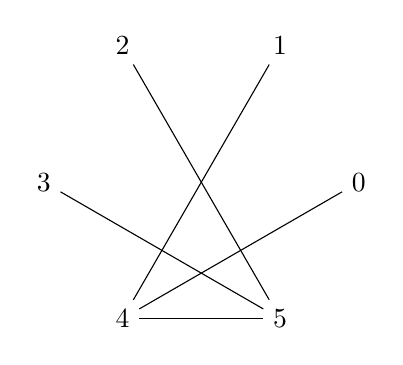
\begin{tikzpicture}
      \draw
        (0.0:2) node (0){0}
        (60.0:2) node (1){1}
        (120.0:2) node (2){2}
        (180.0:2) node (3){3}
        (240.0:2) node (4){4}
        (300.0:2) node (5){5};
      \begin{scope}[-]
        \draw (0) to (4);
        \draw (1) to (4);
        \draw (2) to (5);
        \draw (3) to (5);
        \draw (4) to (5);
      \end{scope}
    \end{tikzpicture}
\end{figure}
\begin{itemize}
\item signature: 000100010001011
\item g: Graph with 6 nodes and 5 edges
\item order: 6
\item size: 5
\item max degree: 3
\item degrees: 1,1,1,1,3,3
\item is tree: 1
\item is bipartite: 1
\item has bridge: 1
\item is chordal: 1
\item is complete: 0
\item min cycle basis weight: 0
\item min cycle basis size: 0
\item diameter: 3
\item radius: 2
\item is eulerian: 0
\item is planar: 1
\item number of faces: 1
\item is regular: 0
\item p3: 6
\item p4: 4
\item property hash: d3c8340b28a64f0a62683dca9f36a56a4802d89a3eeb3c066ff747c4891a74c3
\end{itemize}
\newpage
\begin{figure}
  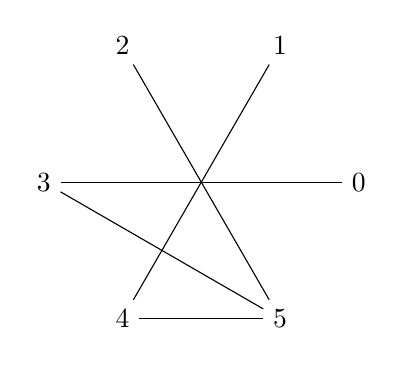
\begin{tikzpicture}
      \draw
        (0.0:2) node (0){0}
        (60.0:2) node (1){1}
        (120.0:2) node (2){2}
        (180.0:2) node (3){3}
        (240.0:2) node (4){4}
        (300.0:2) node (5){5};
      \begin{scope}[-]
        \draw (0) to (3);
        \draw (1) to (4);
        \draw (2) to (5);
        \draw (3) to (5);
        \draw (4) to (5);
      \end{scope}
    \end{tikzpicture}
\end{figure}
\begin{itemize}
\item signature: 001000010001011
\item g: Graph with 6 nodes and 5 edges
\item order: 6
\item size: 5
\item max degree: 3
\item degrees: 1,1,1,2,2,3
\item is tree: 1
\item is bipartite: 1
\item has bridge: 1
\item is chordal: 1
\item is complete: 0
\item min cycle basis weight: 0
\item min cycle basis size: 0
\item diameter: 4
\item radius: 2
\item is eulerian: 0
\item is planar: 1
\item number of faces: 1
\item is regular: 0
\item p3: 5
\item p4: 4
\item property hash: c4b391c168754306af8a50fd5c7d5df582917e6f3ef37e5d521478e253e1cd6a
\end{itemize}
\newpage
\begin{figure}
  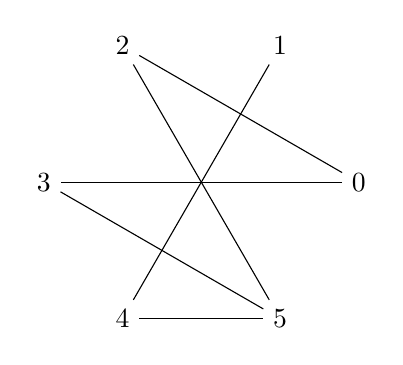
\begin{tikzpicture}
      \draw
        (0.0:2) node (0){0}
        (60.0:2) node (1){1}
        (120.0:2) node (2){2}
        (180.0:2) node (3){3}
        (240.0:2) node (4){4}
        (300.0:2) node (5){5};
      \begin{scope}[-]
        \draw (0) to (2);
        \draw (0) to (3);
        \draw (1) to (4);
        \draw (2) to (5);
        \draw (3) to (5);
        \draw (4) to (5);
      \end{scope}
    \end{tikzpicture}
\end{figure}
\begin{itemize}
\item signature: 011000010001011
\item g: Graph with 6 nodes and 6 edges
\item order: 6
\item size: 6
\item max degree: 3
\item degrees: 1,2,2,2,2,3
\item is tree: 0
\item is bipartite: 1
\item has bridge: 1
\item is chordal: 0
\item is complete: 0
\item min cycle basis weight: 4
\item min cycle basis size: 1
\item diameter: 4
\item radius: 2
\item is eulerian: 0
\item is planar: 1
\item number of faces: 2
\item is regular: 0
\item p3: 7
\item p4: 4
\item property hash: 10c2feecaf5c6ec9fa63b9125ec459f7da42d7c51adc69b520d9245884b6284e
\end{itemize}
\newpage
\begin{figure}
  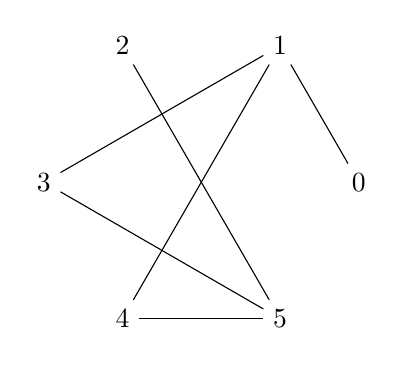
\begin{tikzpicture}
      \draw
        (0.0:2) node (0){0}
        (60.0:2) node (1){1}
        (120.0:2) node (2){2}
        (180.0:2) node (3){3}
        (240.0:2) node (4){4}
        (300.0:2) node (5){5};
      \begin{scope}[-]
        \draw (0) to (1);
        \draw (1) to (3);
        \draw (1) to (4);
        \draw (2) to (5);
        \draw (3) to (5);
        \draw (4) to (5);
      \end{scope}
    \end{tikzpicture}
\end{figure}
\begin{itemize}
\item signature: 100000110001011
\item g: Graph with 6 nodes and 6 edges
\item order: 6
\item size: 6
\item max degree: 3
\item degrees: 1,1,2,2,3,3
\item is tree: 0
\item is bipartite: 1
\item has bridge: 1
\item is chordal: 0
\item is complete: 0
\item min cycle basis weight: 4
\item min cycle basis size: 1
\item diameter: 4
\item radius: 2
\item is eulerian: 0
\item is planar: 1
\item number of faces: 2
\item is regular: 0
\item p3: 8
\item p4: 4
\item property hash: b0278d13cadf5f98ed8fe1e3943a9114e5bf491ae05d4956905101c17585c3d1
\end{itemize}
\newpage
\begin{figure}
  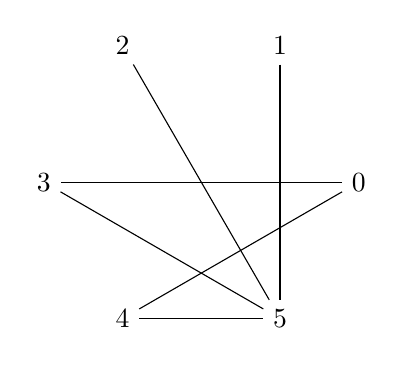
\begin{tikzpicture}
      \draw
        (0.0:2) node (0){0}
        (60.0:2) node (1){1}
        (120.0:2) node (2){2}
        (180.0:2) node (3){3}
        (240.0:2) node (4){4}
        (300.0:2) node (5){5};
      \begin{scope}[-]
        \draw (0) to (3);
        \draw (0) to (4);
        \draw (1) to (5);
        \draw (2) to (5);
        \draw (3) to (5);
        \draw (4) to (5);
      \end{scope}
    \end{tikzpicture}
\end{figure}
\begin{itemize}
\item signature: 001100001001011
\item g: Graph with 6 nodes and 6 edges
\item order: 6
\item size: 6
\item max degree: 4
\item degrees: 1,1,2,2,2,4
\item is tree: 0
\item is bipartite: 1
\item has bridge: 1
\item is chordal: 0
\item is complete: 0
\item min cycle basis weight: 4
\item min cycle basis size: 1
\item diameter: 3
\item radius: 2
\item is eulerian: 0
\item is planar: 1
\item number of faces: 2
\item is regular: 0
\item p3: 9
\item p4: 4
\item property hash: 6bf2ad74343c8cca4ee41f76fe57175dfca4168cd41b3ad0d5fee0bc895537b2
\end{itemize}
\newpage
\begin{figure}
  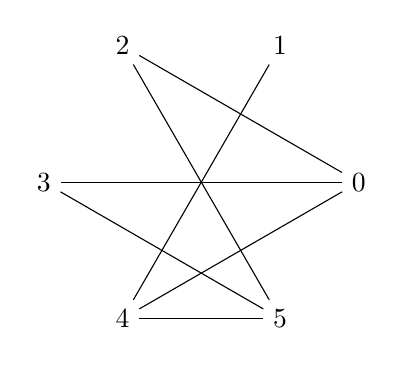
\begin{tikzpicture}
      \draw
        (0.0:2) node (0){0}
        (60.0:2) node (1){1}
        (120.0:2) node (2){2}
        (180.0:2) node (3){3}
        (240.0:2) node (4){4}
        (300.0:2) node (5){5};
      \begin{scope}[-]
        \draw (0) to (2);
        \draw (0) to (3);
        \draw (0) to (4);
        \draw (1) to (4);
        \draw (2) to (5);
        \draw (3) to (5);
        \draw (4) to (5);
      \end{scope}
    \end{tikzpicture}
\end{figure}
\begin{itemize}
\item signature: 011100010001011
\item g: Graph with 6 nodes and 7 edges
\item order: 6
\item size: 7
\item max degree: 3
\item degrees: 1,2,2,3,3,3
\item is tree: 0
\item is bipartite: 1
\item has bridge: 1
\item is chordal: 0
\item is complete: 0
\item min cycle basis weight: 8
\item min cycle basis size: 2
\item diameter: 3
\item radius: 2
\item is eulerian: 0
\item is planar: 1
\item number of faces: 3
\item is regular: 0
\item p3: 11
\item p4: 4
\item property hash: a8f320d2eced901c99384d2c957b4c9b273dcc72954afe74520cedeb6489e6ab
\end{itemize}
\newpage
\begin{figure}
  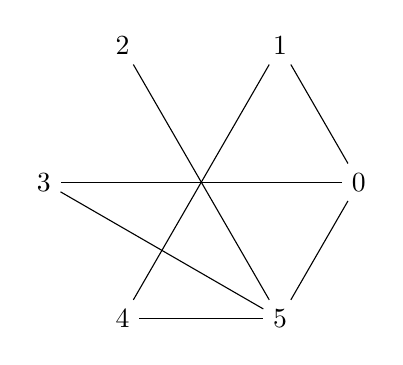
\begin{tikzpicture}
      \draw
        (0.0:2) node (0){0}
        (60.0:2) node (1){1}
        (120.0:2) node (2){2}
        (180.0:2) node (3){3}
        (240.0:2) node (4){4}
        (300.0:2) node (5){5};
      \begin{scope}[-]
        \draw (0) to (1);
        \draw (0) to (3);
        \draw (0) to (5);
        \draw (1) to (4);
        \draw (2) to (5);
        \draw (3) to (5);
        \draw (4) to (5);
      \end{scope}
    \end{tikzpicture}
\end{figure}
\begin{itemize}
\item signature: 101010010001011
\item g: Graph with 6 nodes and 7 edges
\item order: 6
\item size: 7
\item max degree: 4
\item degrees: 1,2,2,2,3,4
\item is tree: 0
\item is bipartite: 0
\item has bridge: 1
\item is chordal: 0
\item is complete: 0
\item min cycle basis weight: 7
\item min cycle basis size: 2
\item diameter: 3
\item radius: 2
\item is eulerian: 0
\item is planar: 1
\item number of faces: 3
\item is regular: 0
\item p3: 9
\item p4: 4
\item property hash: d6bca67354f6d1d7e701ef3379260f28cd4992f4d0285810c6f071a8c2af5d4d
\end{itemize}
\newpage
\begin{figure}
  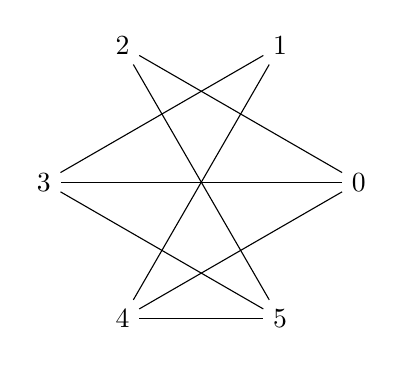
\begin{tikzpicture}
      \draw
        (0.0:2) node (0){0}
        (60.0:2) node (1){1}
        (120.0:2) node (2){2}
        (180.0:2) node (3){3}
        (240.0:2) node (4){4}
        (300.0:2) node (5){5};
      \begin{scope}[-]
        \draw (0) to (2);
        \draw (0) to (3);
        \draw (0) to (4);
        \draw (1) to (3);
        \draw (1) to (4);
        \draw (2) to (5);
        \draw (3) to (5);
        \draw (4) to (5);
      \end{scope}
    \end{tikzpicture}
\end{figure}
\begin{itemize}
\item signature: 011100110001011
\item g: Graph with 6 nodes and 8 edges
\item order: 6
\item size: 8
\item max degree: 3
\item degrees: 2,2,3,3,3,3
\item is tree: 0
\item is bipartite: 1
\item has bridge: 0
\item is chordal: 0
\item is complete: 0
\item min cycle basis weight: 12
\item min cycle basis size: 3
\item diameter: 3
\item radius: 2
\item is eulerian: 0
\item is planar: 1
\item number of faces: 4
\item is regular: 0
\item p3: 14
\item p4: 4
\item property hash: 95839c0fac0daec3d2dd1c483115b25ce7a27c07159808bcc92b54b029886fd6
\end{itemize}
\newpage
\begin{figure}
  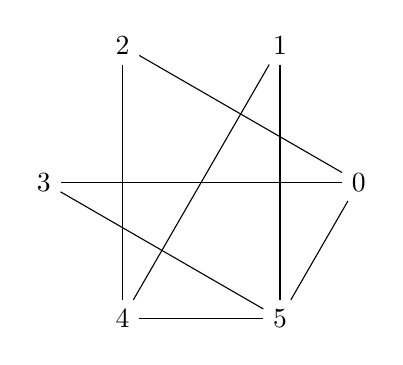
\begin{tikzpicture}
      \draw
        (0.0:2) node (0){0}
        (60.0:2) node (1){1}
        (120.0:2) node (2){2}
        (180.0:2) node (3){3}
        (240.0:2) node (4){4}
        (300.0:2) node (5){5};
      \begin{scope}[-]
        \draw (0) to (2);
        \draw (0) to (3);
        \draw (0) to (5);
        \draw (1) to (4);
        \draw (1) to (5);
        \draw (2) to (4);
        \draw (3) to (5);
        \draw (4) to (5);
      \end{scope}
    \end{tikzpicture}
\end{figure}
\begin{itemize}
\item signature: 011010011010011
\item g: Graph with 6 nodes and 8 edges
\item order: 6
\item size: 8
\item max degree: 4
\item degrees: 2,2,2,3,3,4
\item is tree: 0
\item is bipartite: 0
\item has bridge: 0
\item is chordal: 0
\item is complete: 0
\item min cycle basis weight: 10
\item min cycle basis size: 3
\item diameter: 2
\item radius: 2
\item is eulerian: 0
\item is planar: 1
\item number of faces: 4
\item is regular: 0
\item p3: 9
\item p4: 4
\item property hash: 018104cc750f9fcbcf9ca11114d198d8c0fcd373ff945729a488bc0c9db23e8e
\end{itemize}
\newpage
